\section{Introduction} \label{s:intro}

% start with introduction / motivations of entire HENRI project
The Transient Reactor Test (TREAT) facility, located at the Materials and Fuels Complex at Idaho National Laboratory (INL), is a research reactor with the primary purpose of testing fuels under transient conditions and supporting the development of accident-tolerant fuel \cite{CINBIZ2017}. The reactor can shape these transients using control rods and the negative reactivity temperature feedback, with a maximum energy deposition of \SI{2500}{\mega\joule} \cite{Holschuh2019}. Currently, with this energy deposition limit, the pulse full-width at half-maximum (FWHM) TREAT is capable of generating is around \SI{100}{\milli\second} \cite{Holschuh2019}. This pulse width is outside of the range for a Light Water Reactor (LWR) Reactivity Initiated Accident (RIA) of 30 to \SI{60}{\milli\second} \cite{NEA2010}. A limited number of research reactors are able to produce transient conditions representative of LWRs. \Cref{fig:trans comp} presents a comparison of transient conditions that can be produced by contemporary reactors. There are not any reactors that are able to reproduce the conditions (FWHM and maximum power) of a LWR RIA. The Power Burst Facility (PBF) is the closest to matching the conditions of an LWR RIA, however it has been decommissioned and cannot be used. Using its control rods, TREAT can decrease its transient FWHM down to \SI{89}{\milli\second} \cite{NEA2010}, shown as a red dashed line in \Cref{fig:trans comp}. A further reduction in FWHM would bring TREAT near BWR conditions.



% transient reactor comparison plot -- ripped from source paper by Bess -- look for the one Mignot used in the old nureth paper
\begin{figure}[htbp]
    \vspace{16pt}
    \centering
    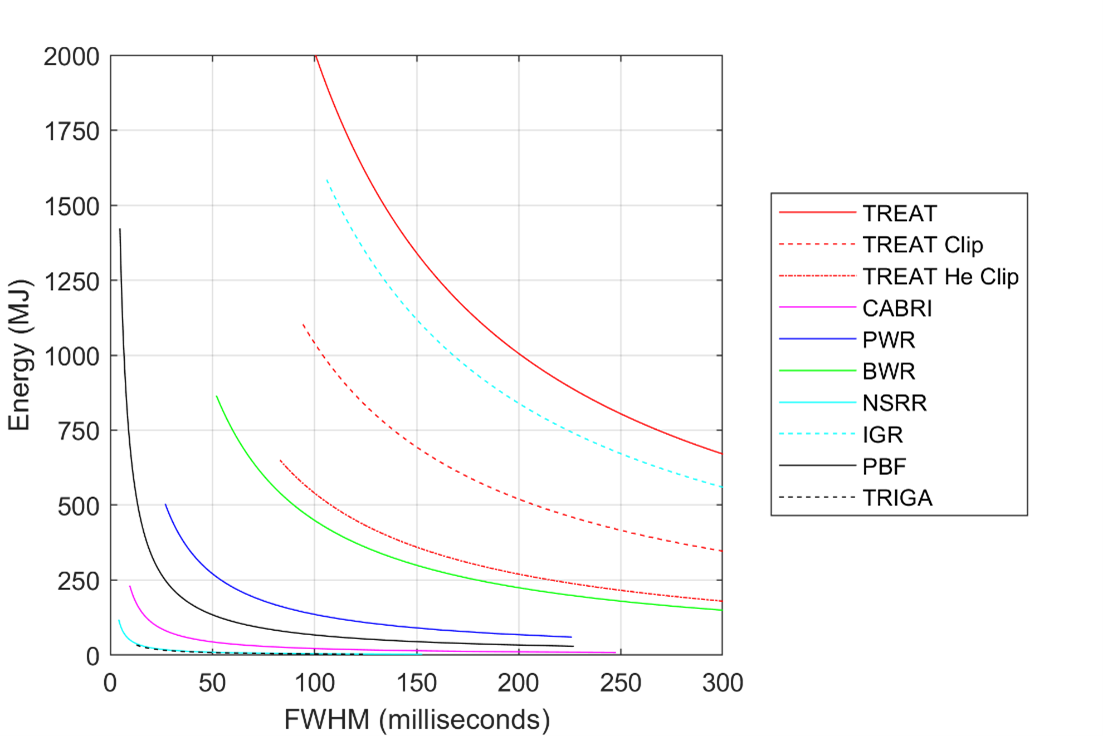
\includegraphics[width=0.75\textwidth]{intro/plots/ReactorTransientComp_Kevin.png}
    \caption{Comparison of contemporary reactor transient conditions \cite{BESS2019}.}
    \label{fig:trans comp}
    \vspace{16pt}
\end{figure}


Crawford \cite{Crawford1998} suggested the use of helium-3, a strong neutron absorber gas, for clipping a high-power pulse in TREAT. Such a system would be capable of inserting a negative reactivity of -5\% $\Delta k/k$ without the use of control rods. The original calculation results in a FWHM reduced to 40-\SI{60}{\milli\second} for a total energy deposition of \SI{1600}{\mega\joule}, well below the \SI{2500}{\mega\joule} limit, and the peak power was estimated to be \SI{20000}{\mega\watt}. This pulse is more representative of the postulated LWR RIA and is shown as a red dotted line in \Cref{fig:trans comp}.

Helium-3 has been used for a similar purpose at the CABRI reactor in Cadarache, France. At CABRI, helium-3 is pressurized in 4 tubes in the core, then to initiate a transient, the helium-3 is rapidly depressurized from the core (negative reactivity removal). This depressurization is precisely controlled using multiple valves to produce the desired pulse width and power for the transient \cite{Clamens2016,Clamens2018,Clamens2018b}. In TREAT, this process will be reversed by rapidly pressurizing tubes in the core with helium-3 to shut down a transient (negative reactivity insertion). CABRI has been updated and is currently used under the OECD/NEA CABRI International Project (CIP).

Initial calculations for the TREAT facility showed that a helium-3 pressure of \SI{1.72}{\mega\pascal} (\SI{250}{psi}) in a cartridge volume of \SI{1167}{\centi\meter^3} would be sufficient to reach the desired negative reactivity of -5\% $\Delta k/k$. This pressure corresponds to an atomic density of \SI{3.35e20}{atoms\per\centi\meter^3}. For a pulse to be clipped properly, it is estimated that the helium-3 must be injected in \SI{5}{\milli\second} \cite{BESS2019}. Oregon State University (OSU) was tasked to model, design, and test an out-of-pile prototype cartridge to assess the feasibility and repeatability of the physical process; and identify and solve any engineering issues associated with the device. The experimental Helium-3 Negative Reactivity Insertion (HENRI) facility was designed and built at OSU. Testing was performed to determine the feasibility and repeatability of the gas injection, with positive results \cite{HeNURETH}. This paper presents updates to the HENRI facility, as well as continued work in the experimental campaign, specifically focusing on the development and testing of a bespoke fast-opening valve for the facility.



% describe the need for a new fast-opening valve -- should this be its own section?
\subsection{Need for a Fast-opening Valve} \label{s:need for valve}

The previous work on HENRI at OSU \cite{HeNURETH} used rupture disks to characterize the system and its physics. Rupture disks provided an almost instantaneous opening, which allowed for the gas physics to be isolated and compared against CFD models \cite{CFDNureth}. The rupture disks, however, have major drawbacks for use in the HENRI system for TREAT. Firstly, the rupture disks must be changed after each use, which would mean taking the HENRI system out of the TREAT reactor and dealing with the radiation of the system before changing the rupture disk and reinstalling the system in the reactor. This process adds danger and complexity, on top of the time, to a system intended to be utilized heavily during RIA testing campaigns. Secondly, the rupture disks do not rupture in a predictable manner. There is tolerance in the manufacture of rupture disks that causes the disks to rupture at slightly different pressures, which is not ideal when the system needs to be precisely timed with the peak of a transient. These problems with the rupture disk have lead OSU to investigate a more permanent valve option. This valve must be reusable, precise, fast-opening, and durable. The valve must also fit into the physical space constraints of the HENRI system, which includes its power or actuation method, and not contaminate the helium-3 used in the system.


